\chapter{Классификация существующих\newline методов решения}

В данном разделе будут описаны существующие методы решения, выделены критерии их оценки, и будет проведено сравнение описанных методов по выделенным критериям.

\section{Методы решения}

Существуют следующие методы изменения ядра Linux:

\begin{itemize}
	\item требующие перезагрузки системы;
	\item переноса;
	\item динамические.
\end{itemize}

\subsection{Методы, требующие перезагрузки системы}

Первые применения патчей к ядру происходили по следующему алгоритму \cite{dwarf}:

\begin{itemize}
	\item работающие приложения закрываются;
	\item происходит загрузка и инициализация исправленного ядра;
	\item приложения перезагружаются.
\end{itemize}

Так, неисправленное ядро заменялось исправленным ядром. 

В процессе внесения изменений в ядро операционной системы описанным способом возникает следующая проблема: появляется время простоя, которое состоит из времени простоя приложения и простоя ядра, что показано на рисунке \ref{img:downtime}.

\begin{figure}[H]
	\begin{center}
		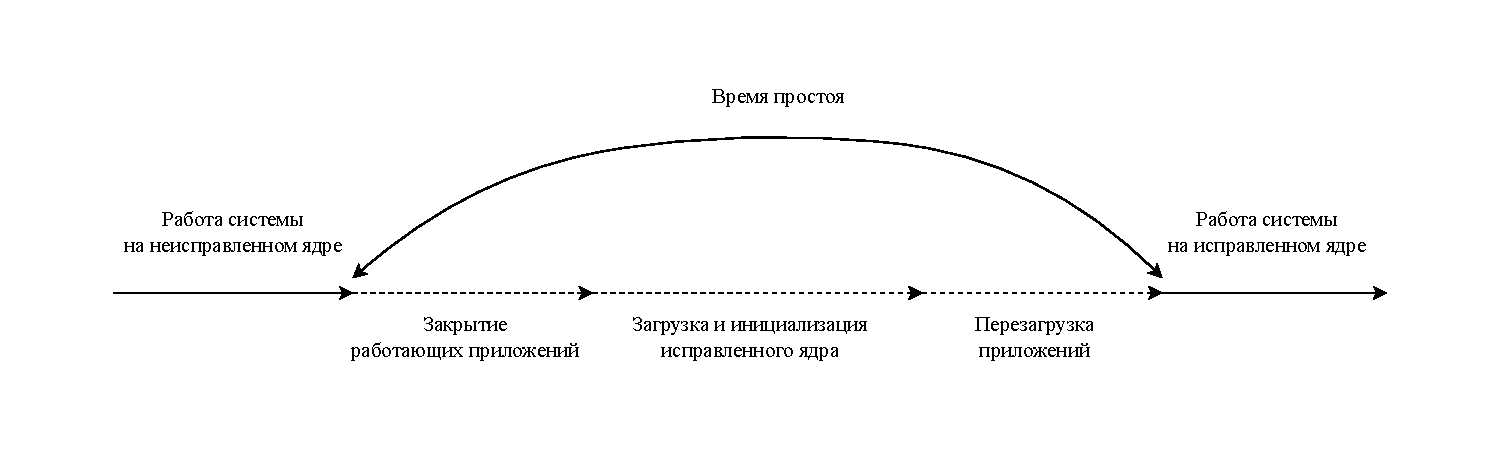
\includegraphics[scale=0.7]{img/downtime.pdf}
	\end{center}
	\captionsetup{justification=centering}
	\caption{Время простоя при перезагрузке системы}
	\label{img:downtime}
\end{figure}

Для снижения времени простоя появились модификации метода, которые эффективно управляют перезагрузкой ядра. Одно из решений - метод контрольной точки \cite{kup}.

В данном методе используется системный вызов $kexec$  \cite{seamless} для загрузки нового образа ядра. Этот механизм позволяет загружать новое ядро из работающего в данный момент ядра в основную память и сразу же начинает его выполнение.

Чтобы применить патч необходимо дождаться момента, когда система примет состояние, в котором выполнены два условия:
\begin{itemize}
	\item все потоки ядра остановлены;
	\item структуры данных ядра согласованны.
\end{itemize}

Выполнение этих двух условий позволяет сделать контрольную точку, которая позволяет сохранить состояние приложений. Контрольная точка сохраняет состояния процессов, состоящих из их пространства памяти (разделы кода или данных, стека или кучи)
и их внутренние состояния в ядре. Код контрольной точки проходит через структуры данных ядра, связанные с приложениями, и преобразует их в высокоуровневый формат, который не зависит от версии ядра. 

После сохранения контрольной точки выполняется инициализация нового ядра. Исправленное ядро считывает контрольную точку и восстанавливает приложения, а затем перезапускает их.

Техника этого метода показана на рисунке \ref{img:checkpoint}.

\begin{figure}[H]
	\begin{center}
		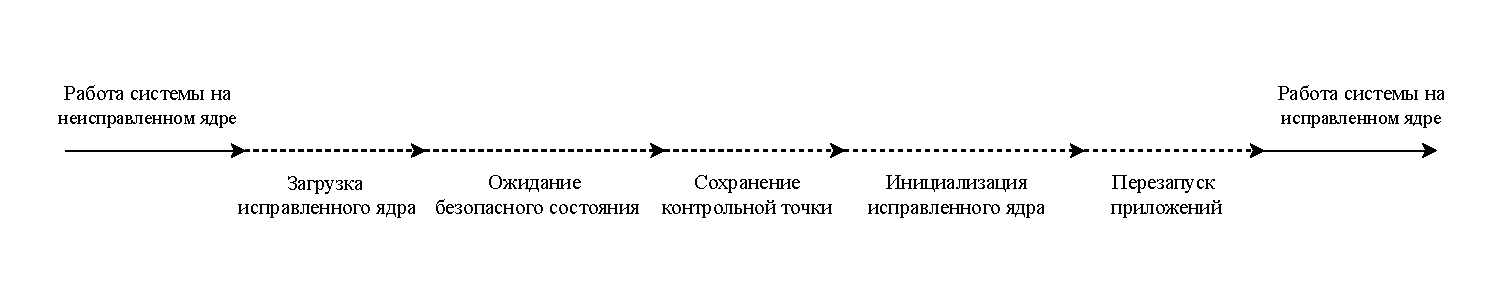
\includegraphics[scale=0.7]{img/checkpoint.pdf}
	\end{center}
	\captionsetup{justification=centering}
	\caption{Метод контрольной точки}
	\label{img:checkpoint}
\end{figure}

Существует метод, который сокращает время простоя путем одновременного выполнения приложений и перезагрузки системы - метод теневой перезагрузки \cite{shadow}. Перезагрузка операционной системы выполняется в фоновом режиме на виртуальной машине. Приложения могут продолжать выполняться на исходной машине.

После перезагрузки ядра на выделенной виртуальной машине, делается снимок системы, из которого восстанавливается файловая система на исходной машине.

Во время теневой перезагрузки пользовательские приложения могут изменять файлы исходной машины. Файлы могут быть изменены и на выделенной виртуальной машине. Так как файловая система восстанавливается из снимка, то изменения файлов на исходной машине теряются. То есть, файловая система откатывается до состояния, когда создавалась выделенная виртуальная машина.

Для согласованности файлов в методе теневой перезагрузки вводят понятие срока перезагрузки, в течение которого пользователи могут изменять файлы каталогов. Срок перезагрузки - это период, который начинается с создания выделенной виртуальной машины и завершается после создания снимка выделенной виртуальной машины. При восстановлении файловой системы сохраняются файлы, измененные во время срока перезагрузки на исходной машине, и добавляются другие файлы выделенной виртуальной машины. 

Описанный метод представлен на рисунке \ref{img:shadow-reboot}.

\begin{figure}[H]
	\begin{center}
		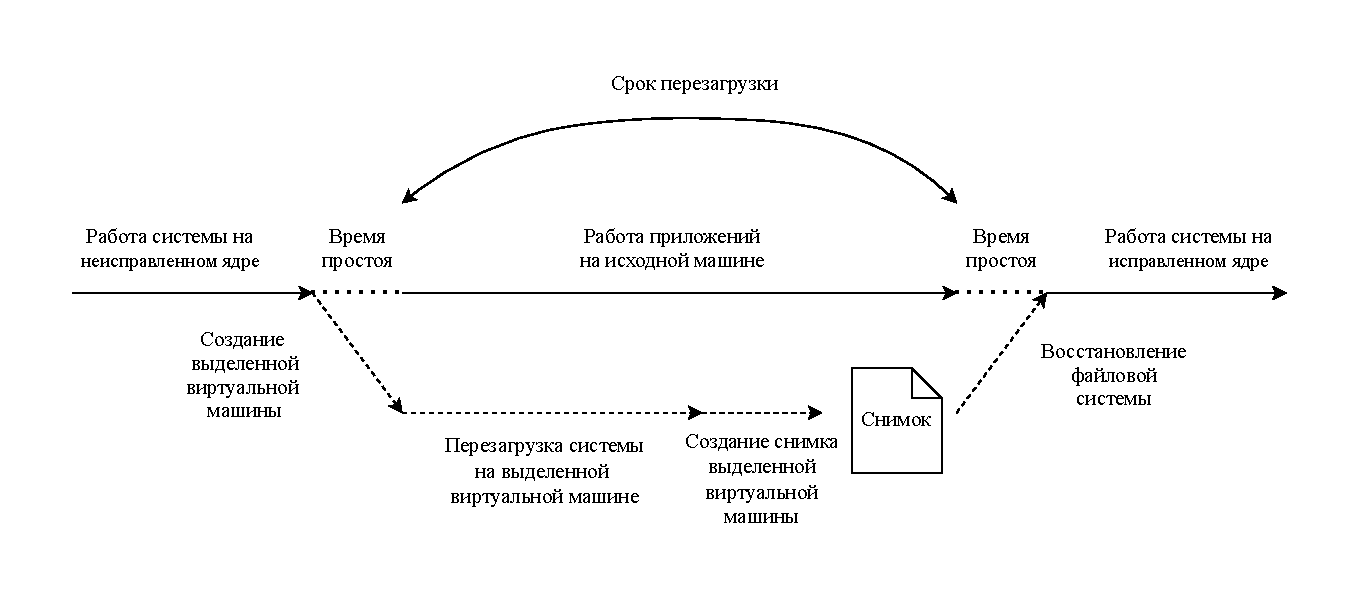
\includegraphics[scale=0.7]{img/shadow-reboot.pdf}
	\end{center}
	\captionsetup{justification=centering}
	\caption{Метод теневой перезагрузки}
	\label{img:shadow-reboot}
\end{figure}

Плюсом данных методов является отсутсвие необходимости дополнительных машин или общих хранилищ.

Метод теневой перезагрузки приводит к простою приложения, а метод контрольной точки восстановление процесса не может выполняться до тех пор, пока не завершится перезапуск ядра операционной системы, что приведет к простою ядра. Перезагрузка может привести к потере доступности критических задач или процессов, работающих в этой операционной системе.

Следующие методы решают проблему простоя исключением перезагрузки системы.

\subsection{Метод переноса}

Идея данного метода \cite{autopod} заключается в следующем: на дополнительной машине запускается измененное ядро, на него переносятся запущенные процессы старого ядра, и оно останавливается. Так как использование дополнительной физической машины ресурсозатратно, в существующих решениях \cite{lucos} в качестве допольнительной машины используется виртуальная машина, установленная на физической машине, требующей обновления ядра. Необходимо общее хранилище (сервер), которое подключено и к старому, и к новому ядрам. Патч применяется в три этапа.

На первом этапе собирается информация о состоянии операционной системы: подсчитывается число потоков, выполняемых в исправляемом коде, вызывается функция запуска, выполняется инициализация перед передачей управления виртуальной машине.

На втором этапе начинается исправление структур данных и функций. Если не измененный модуль используется, обе версии структур данных должны существовать во время процесса исправления. Для обеспечения согласованности структур данных, страницы исходных данных и новых данных защищены. Перехват доступа к ним контролируется виртуальной машиной. То есть, при попытке изменить отслеживаемую страницу управление будет передано виртуальной машине. В этот момент сравнивается содержимое двух версий и вызывается функция передачи состояния, как показано на рисунке \ref{img:vm}.

\begin{figure}[H]
	\begin{center}
		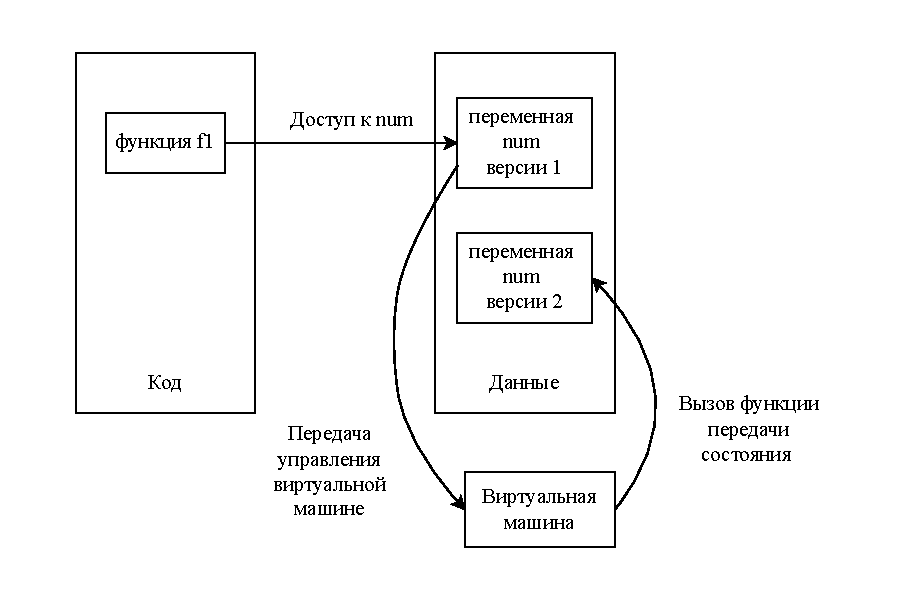
\includegraphics[scale=0.8]{img/vm.pdf}
	\end{center}
	\captionsetup{justification=centering}
	\caption{Согласованность данных в методе переноса}
	\label{img:vm}
\end{figure}

На последнем этапе отключается контроль исходных структур данных. Для этого используется метод обхода стека. В случае, если соответствующая исходные структуры используются, адрес возврата исходной функции заменяется адресом функции-заглушки, которые позволяют определить, используется ли еще обновленная функция. Затем выполняется очистка кода старой версии и устанавливается флаг завершения патчинга.

При применении данного метода время простоя невелико. Главным минусом является высокое потребление ресурсов центрального процессора, сети и объема памяти.

\subsection{Динамические методы}

Данные методы \cite{ksplice} \cite{dynamos} позволяют применять патчи во время выполнения процессов без перезагрузки и дополнительных ресурсов. Решение состоит из двух этапов, показанных на рисунке \ref{img:dynamic}.

Для того, чтобы создать измененный код, проводится анализ обновленной и старой	версий. Для этого собирается два варианта ядра: сборка исходного кода и сборка измененного кода. Файлы, полученные сборкой неизмененного кода называют предварительными объектными файлами, файлы, полученные в результате сборки кода патча - последующими объектными файлами. В отличие от поиска различий в исходном коде, анализ объектного кода позволяет понять, какие функции были изменены в патче. Большинство функций ядра, которые не были изменены патчем, будут иметь одинаковые объектные коды. Обнаруженные измененные функции помещаются в основной модуль для загрузки в ядро.

\begin{figure}[H]
	\begin{center}
		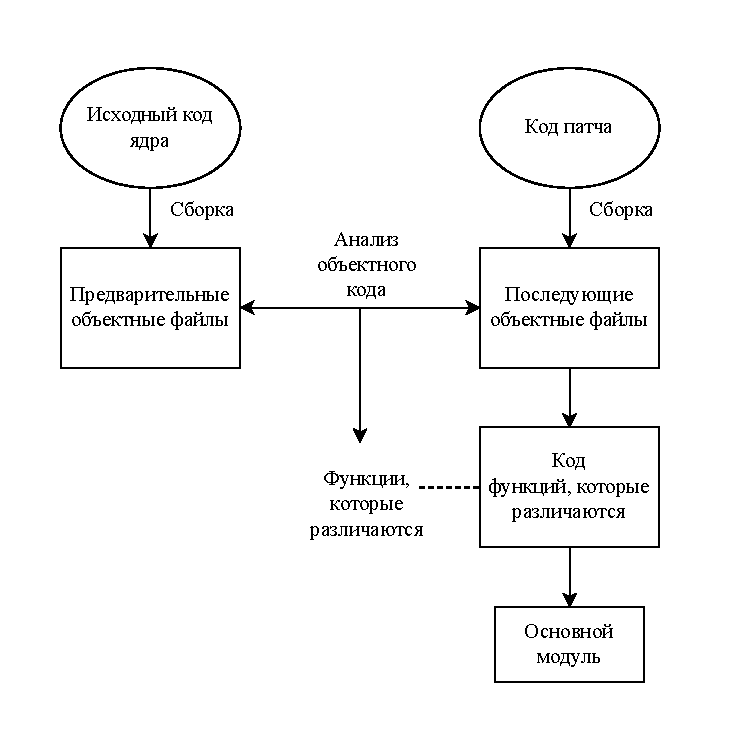
\includegraphics[scale=0.8]{img/dynamic.pdf}
	\end{center}
	\captionsetup{justification=centering}
	\caption{Динамический метод}
	\label{img:dynamic}
\end{figure}

Следующий этап необходим для обнаружения встраиваемых функций и неуникальных символов. Для этого проводится сравнение работающего кода ядра и скомпилированного кода. Этот процесс называется предварительным сопоставлением.

Для применения данного метода необходимо определить состояние ядра, когда каждая заменяемая функция будет находиться в состоянии покоя, что является условием безопасного внесения изменений. В этом случае модуль может быть загружен в ядро. Проверка условия безопасного внесения изменений в случае неудачи возобновится через некоторое время. После нескольких неудачных попыток достичь безопасного состояния для применения патча процесс прерывается. Новые инструкции будут вставлены в необновленные функции путем бинарной перезаписи. Бинарная перезапись - это перенаправление вызова функции из исходной в исправленную, для чего используется прыжок к первым пяти или шести байтам функции.

Данные методы решают проблему с временем простоя.

Решения на основе динамических методов не поддерживают семантические изменения. Кроме того, возникают сложности с изменением типов и структур данных, нестабильных типов данных и функций ядра, которые всегда находятся в стеке вызовов потоков ядра.

\section{Критерии оценки методов}

Сравнение описанных методов изменения ядра Linux будет проводиться по следующим критериям:

\begin{itemize}
	\item необходимость перезагрузки;
	\item наличие времени простоя;
	\item возможность семантических изменений;
	\item потребление ресурсов.
\end{itemize}

\section{Сравнение методов}

Обозначим введенные критерии оценки методов следующим образом:

\begin{itemize}
	\item К1 - необходимость перезагрузки системы;
	\item К2 - наличие времени простоя;
	\item К3 - возможность семантических изменений;
	\item К4 - потребление ресурсов.
\end{itemize}

Результаты сравнения методов изменения ядра Linux представлены в таблице \ref{tab:comparison}.

\begin{table}[h]
    \caption{Сравнение методов изменения ядра Linux}
    \begin{center}
        \begin{tabular}{|c|c|c|c|c|}
            \hline
            Метод & К1 & К2 & К3 & К4 \\ \hline
            Контрольной точки & необходима & есть & есть & 100 \% \\ \hline
            Теневой перезагрузки & необходима & есть & есть & 100 \% \\ \hline
            Переноса & отсутствует & есть & есть & 200 \% \\ \hline
            Динамический & отсутствует & нет & нет & 100 \% \\ \hline
        \end{tabular}
    \end{center}
    \label{tab:comparison}
\end{table}

По результатам сравнения самым эффективным методом внесения изменений в ядро Linux оказался динамический метод. Главными недостаткамми методов контрольной точки и теневой перзагрузки являются необходимость перезагрузки системы и наличие времени простоя. В методе переноса перезагрузка системы не требуется и время простоя снижено, но потребление ресурсов увеличивается в два раза. Кроме того методы, требующие перезагрузки системы, и метод переноса восполняют недостаток динамического метода - отсутствие возможности внесения семантических изменений.

\section{Вывод}

В данном разделе были рассмотрены существующие методы решения, выделены критерии их оценки, а также было проведено сравнение описанных методов по выделенным критериям.
